\documentclass[journal,12pt,twocolumn]{IEEEtran}

\usepackage{setspace}
\usepackage{gensymb}
\singlespacing
\usepackage[cmex10]{amsmath}

\usepackage{amsthm}

\usepackage{mathrsfs}
\usepackage{txfonts}
\usepackage{stfloats}
\usepackage{bm}
\usepackage{cite}
\usepackage{cases}
\usepackage{subfig}

\usepackage{longtable}
\usepackage{multirow}

\usepackage{enumitem}
\usepackage{mathtools}
\usepackage{steinmetz}
\usepackage{tikz}
\usepackage{circuitikz}
\usepackage{verbatim}
\usepackage{tfrupee}
\usepackage[breaklinks=true]{hyperref}
\usepackage{graphicx}
\usepackage{tkz-euclide}

\usetikzlibrary{calc,math}
\usepackage{listings}
    \usepackage{color}                                            %%
    \usepackage{array}                                            %%
    \usepackage{longtable}                                        %%
    \usepackage{calc}                                             %%
    \usepackage{multirow}                                         %%
    \usepackage{hhline}                                           %%
    \usepackage{ifthen}                                           %%
    \usepackage{lscape}     
\usepackage{multicol}
\usepackage{chngcntr}

\DeclareMathOperator*{\Res}{Res}

\renewcommand\thesection{\arabic{section}}
\renewcommand\thesubsection{\thesection.\arabic{subsection}}
\renewcommand\thesubsubsection{\thesubsection.\arabic{subsubsection}}

\renewcommand\thesectiondis{\arabic{section}}
\renewcommand\thesubsectiondis{\thesectiondis.\arabic{subsection}}
\renewcommand\thesubsubsectiondis{\thesubsectiondis.\arabic{subsubsection}}


\hyphenation{op-tical net-works semi-conduc-tor}
\def\inputGnumericTable{}                                 %%

\lstset{
%language=C,
frame=single, 
breaklines=true,
columns=fullflexible
}
\begin{document}

\newcommand{\BEQA}{\begin{eqnarray}}
\newcommand{\EEQA}{\end{eqnarray}}
\newcommand{\define}{\stackrel{\triangle}{=}}
\bibliographystyle{IEEEtran}
\raggedbottom
\setlength{\parindent}{0pt}
\providecommand{\mbf}{\mathbf}
\providecommand{\pr}[1]{\ensuremath{\Pr\left(#1\right)}}
\providecommand{\qfunc}[1]{\ensuremath{Q\left(#1\right)}}
\providecommand{\sbrak}[1]{\ensuremath{{}\left[#1\right]}}
\providecommand{\lsbrak}[1]{\ensuremath{{}\left[#1\right.}}
\providecommand{\rsbrak}[1]{\ensuremath{{}\left.#1\right]}}
\providecommand{\brak}[1]{\ensuremath{\left(#1\right)}}
\providecommand{\lbrak}[1]{\ensuremath{\left(#1\right.}}
\providecommand{\rbrak}[1]{\ensuremath{\left.#1\right)}}
\providecommand{\cbrak}[1]{\ensuremath{\left\{#1\right\}}}
\providecommand{\lcbrak}[1]{\ensuremath{\left\{#1\right.}}
\providecommand{\rcbrak}[1]{\ensuremath{\left.#1\right\}}}
\theoremstyle{remark}
\newtheorem{rem}{Remark}
\newcommand{\sgn}{\mathop{\mathrm{sgn}}}
\providecommand{\abs}[1]{\vert#1\vert}
\providecommand{\res}[1]{\Res\displaylimits_{#1}} 
\providecommand{\norm}[1]{\lVert#1\rVert}
%\providecommand{\norm}[1]{\lVert#1\rVert}
\providecommand{\mtx}[1]{\mathbf{#1}}
\providecommand{\mean}[1]{E[ #1 ]}
\providecommand{\fourier}{\overset{\mathcal{F}}{ \rightleftharpoons}}
%\providecommand{\hilbert}{\overset{\mathcal{H}}{ \rightleftharpoons}}
\providecommand{\system}{\overset{\mathcal{H}}{ \longleftrightarrow}}
	%\newcommand{\solution}[2]{\textbf{Solution:}{#1}}
\newcommand{\solution}{\noindent \textbf{Solution: }}
\newcommand{\cosec}{\,\text{cosec}\,}
\providecommand{\dec}[2]{\ensuremath{\overset{#1}{\underset{#2}{\gtrless}}}}
\newcommand{\myvec}[1]{\ensuremath{\begin{pmatrix}#1\end{pmatrix}}}
\newcommand{\mydet}[1]{\ensuremath{\begin{vmatrix}#1\end{vmatrix}}}
\numberwithin{equation}{subsection}
\makeatletter
\@addtoreset{figure}{problem}
\makeatother
\let\StandardTheFigure\thefigure
\let\vec\mathbf
\renewcommand{\thefigure}{\theproblem}
\def\putbox#1#2#3{\makebox[0in][l]{\makebox[#1][l]{}\raisebox{\baselineskip}[0in][0in]{\raisebox{#2}[0in][0in]{#3}}}}
     \def\rightbox#1{\makebox[0in][r]{#1}}
     \def\centbox#1{\makebox[0in]{#1}}
     \def\topbox#1{\raisebox{-\baselineskip}[0in][0in]{#1}}
     \def\midbox#1{\raisebox{-0.5\baselineskip}[0in][0in]{#1}}
\vspace{3cm}
\title{AI1103-Assignment 6}
\author{Name : Ayush Jha \\ Roll Number: CS20BTECH11006}
\maketitle
\newpage
\bigskip
\renewcommand{\thefigure}{\theenumi}
\renewcommand{\thetable}{\theenumi}
Download all python codes from 
\begin{lstlisting}
https://github.com/ayushjha2612/AI11003/tree/main/Assignment6/Codes
\end{lstlisting}
%
and latex-tikz codes from 
%
\begin{lstlisting}
https://github.com/ayushjha2612/AI11003/tree/main/Assignment6
\end{lstlisting}
\section{GATE 2021(ST) Q.22 (Statistics section)}
Let X be a random variable having probability density function 
\begin{align*}
\label{eq:qpdf_X}
f\brak{x} = 
\begin{cases}
\frac{3}{13}(1-x)(9-x) & 0 < x < 1
\\
0 & \text{ otherwise}
\end{cases}
\end{align*}
Then $\dfrac{4}{3} E [X(X^2 -15X + 27 ) ] $ equals --- ( round of to two decimal places). \\
\section{Answer}
8.67
\section{Solution}
Let X be the random variable. To find 
\begin{align}
    \frac{4}{3} E[X(X^2 -15X + 27)]
\end{align}
Let,
\begin{align}
    g(X) &= X(X^2 -15X + 27)  \\
         &= X^3 -15X^2 + 27X
\end{align}
Then for random variable X we have that,
\begin{align}
    E[g(X)] = \int_{-\infty}^{\infty} g(x)f(x) \,dx
\end{align}
The probability distribution of X is,
\begin{align}
\label{eq:spdf_X}
f\brak{x} = 
\begin{cases}
\frac{3}{13}(1-x)(9-x) & 0 < x < 1
\\
0 & \text{ otherwise}
\end{cases}
\end{align}
Using \ref{eq:spdf_X} we have,
\begin{align}
    E[g(X)] &= 0 +\int_{0}^{1} g(x)f(x) \,dx + 0
\end{align}
Where ,
\begin{align}
    f(x ) &= \frac{3}{13}(1-x)(9-x) \text{ and}  \\
    g(x) &= x^3 -15x^2 + 27x
\end{align}
Using Integration by substitution let,
\begin{align*}
    t &= x^3 - 15x^2 + 27x \\
    \,dt &= 3x^2 - 30x + 27 \\
         &= 3(1-x)(9-x)
\end{align*}
The corresponding limits are,
\begin{align}
    \text{For } x &=0  \implies t = 0^3 -15\times 0^2 + 27 \times 0 = 0 \\
        \text{For } x &=1  \implies t = 1^3 -15\times 1^2 + 27 \times 1 = 13
\end{align}
Therefore we have,
\begin{align}
    E[g(X)] &= \frac{1}{13} \int_{0}^{13} t \,dt \\
    & = \frac{1}{13} \times \brak{\frac{t^2}{2}}  \Biggr|_{0}^{13} \\
    &= \frac{1}{13} \times \frac{13^2}{2} \\
    & = \frac{13}{2} 
\end{align}
Thus, 
\begin{align}
    \frac{4}{3} E[g(X)] & =  \frac{4}{3} \times \frac{13}{2} \\
    &= \frac{26}{3} \\
    &= 8.67  \text{ (rounded off)}
\end{align}
Therefore,
\begin{align}
    \frac{4}{3} E[X(X^2 -15X + 27)] & =  8.67
\end{align}
The plot for PDF of $X $ can be observed at figure \ref{fig:The PDF of X}. 
\begin{figure}[!ht]
       \centering
    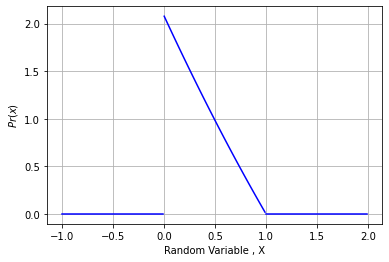
\includegraphics[width=.9\columnwidth] {Assignment_6.png}
    \caption{The PDF of X}
    \label{fig:The PDF of X}
\end{figure}
\end{document}